\documentclass[letterpaper]{article}
\usepackage{flairs}%aaai
\usepackage{times}
\usepackage{helvet}
\usepackage{courier}
\usepackage{amsmath}
\usepackage{amsfonts}
\usepackage{amssymb}
\usepackage{amsthm}
\usepackage{booktabs} 
\usepackage{graphicx}

\usepackage{tikz} % for tikz :) 
\usetikzlibrary{fit} % for fitting the plate
\tikzset{>=latex} % Sets the arrow style

\usepackage{todonotes}
\frenchspacing
\setlength{\pdfpagewidth}{8.5in}
\setlength{\pdfpageheight}{11in}
% Allow \citet style as also done in https://aaai.org/ocs/index.php/FLAIRS/FLAIRS20/paper/view/18398/17511
\newcommand{\citet}[1]{\citeauthor{#1} (\citeyear{#1})}
%% dashed rules for tables from https://www.latex4technics.com/?note=2BGI
\newcommand{\dashrule}[1][black]{%
  \color{#1}\rule[\dimexpr.5ex-.2pt]{4pt}{.4pt}\xleaders\hbox{\rule{4pt}{0pt}\rule[\dimexpr.5ex-.2pt]{4pt}{.4pt}}\hfill\kern0pt%
}
\pdfinfo{
/Title (Modeling and Mitigating Gender Bias in Matching Problems: A Simulation-Based Approach with Quota Constraints)
/Author (Anonymous)}
\setcounter{secnumdepth}{0}  
 \begin{document}
% This file is an adoption of the style file for AAAI Press 
% proceedings, working notes, and technical reports.  This file is made 
% with minimal changes by explicit permission from AAAI.
\title{Modeling and Mitigating Gender Bias in Matching Problems:\\ A~Simulation-Based Approach with Quota Constraints}
\author{Florian Wilhelm\\
inovex GmbH\\
76131 Karlsruhe, Germany\\
\And Anja Pilz\\
Damedic GmbH\\
50677 Cologne, Germany\\ % how detailed should that be?
}

% Add data generating process, explain it
% mention that job capacities don't really change a thing.

\maketitle
\begin{abstract}
\begin{quote}
In high-stakes matching scenarios, such as hiring or resource distribution, biases tied to protected attributes, such as gender, can compromise fairness and efficiency. We propose a simulation-based framework to study the interplay between gender bias and quota policies in many-to-one matching problems, where individuals have preferences over positions with fixed capacities. Individuals' preferences are sampled from gender-specific Dirichlet priors, and we introduce a bias term to favor males artificially. Quotas are incorporated as constraints that ensure a specified female representation. We systematically analyze how bias levels and preference divergence, measured by Total Variation Distance, interact with different quota rules to affect gender-specific and overall efficiency. Our results highlight trade-offs between fairness and total efficiency, demonstrating that carefully calibrated quotas can mitigate disparities while maintaining acceptable efficiency levels. 
\end{quote}
\end{abstract}

\section{Introduction}
Artificial intelligence (AI) systems are increasingly deployed in high-stakes decision-making domains such as hiring, workforce management, and resource allocation. These systems must balance competing objectives, notably efficiency and fairness. Fairness, as an ethical principle, is inherently broad and complex and may never be fully realizable, as suggested by \citet{Peterson_Hamrouni_2022}. However, specific aspects of fairness are legally mandated through regulations such as anti-discrimination laws. The Universal Declaration of Human Rights \cite{udhr1948} explicitly prohibits discrimination based on attributes such as race, color, gender, language, religion, political opinion, or social origin. While this declaration serves as a normative framework for assigning individuals to positions (e.g., jobs or roles), it remains extremely difficult to verify the absence of bias concerning legally protected attributes during the matching process.

A practical method to mitigate biases that lead to discrimination is the implementation of quotas, which are commonly used to address gender disparities. However, similar to the challenge of quantifying biases, evaluating the effectiveness of quotas in mitigating discrimination is equally difficult due to their counterfactual nature. In this work, we focus on a simplified job matching setting based on a binary notion of gender (female \& male). A set of individuals competes for positions with limited capacities. Individuals' preferences reflect their interests and implied abilities according to the Interest-Ability Hypothesis~\cite{jintelligence10030043}. We introduce a bias that artificially inflates one group's attractiveness in the matching process. We measure the overall and group-specific efficiency based on the degree to which the unbiased preferences of the individuals are satisfied. We incorporate quotas via linear constraints on the proportion of female hires, allowing us to explore various levels of enforced female representation. 

Our key contribution is a comprehensive mathematical framework that enables simulation and analysis of the interplay among bias, quotas, and matching efficiencies in many-to-one matching problems. Specifically, we incorporate \textit{Total Variation Distance} (TVD) to control how strongly male and female preferences diverge, allowing a systematic exploration of the effects of bias parameters on fairness and overall optimality. In addition, we propose a novel preference-based quota mechanism that aggregates individual votes to approximate group interests, offering a flexible alternative to static threshold quotas, which perform consistently better while being nearly independent of TVD.

\section{Related Work}

Quotas have been explored as a tool to address group disparities in matching problems. 
\citet{Bertsimas2012OnTE} analyzed the trade-offs between proportional representation (fairness) and overall efficiency in various resource allocation settings, offering insights into how quota-like constraints can shape outcomes. 
Preference-driven fairness mechanisms, such as those introduced by \citet{AzizW14}, align allocations with group-specific priorities, providing a foundation for dynamic, strategy-proof approaches.
Our work extends these investigations by (1) quantifying preference divergence between groups via TVD and (2) proposing a novel preference-based quota mechanism that incorporates these divergent preferences, thereby offering a more flexible approach to balancing 
fairness and efficiency in many-to-one matching scenarios.


\section{Mathematical Model}

Let \( S = \{s_1, \ldots, s_n\} \) be the set of individuals and \( G = \{f, m\} \) the binary set of genders, where \( f \) denotes female and \( m \) denotes male. The set of available positions is \( O = \{o_1, \ldots, o_m\} \), and we introduce the \textit{outside option} \( \emptyset \) to represent the state where an individual remains unmatched. Each position \( o_j \in O \) has a capacity \( c_j = c(o_j) \in \mathbb{N} \), and each individual \( s_i \in S \) is assigned a gender \( g_i = g(s_i) \in G \).

A matching is a function \( \mu : S \to O \cup \{\emptyset\} \) that satisfies:
\begin{enumerate}
    \item \( \mu(s) \in O \cup \{\emptyset\} \) for all \( s \in S \),
    \item  \( |\mu^{-1}(o)| \leq c(o) \) for all \( o \in O \), where \( \mu^{-1}(o) = \{ s \in S \mid \mu(s) = o \} \),
    \item \( \mu(s) = o \iff s \in \mu^{-1}(o) \) for all \( s \in S \) and \( o \in O \).
\end{enumerate}

Each individual \( s_i \) has a preference function \( U_i : O \to [0, 1] \) reflecting how much they prefer each position, with \( \sum_{o_j \in O} U_i(o_j) = 1 \). In line with the \textit{Interest-Ability Hypothesis}~\cite{jintelligence10030043}, preferences are assumed to directly correspond to an individual's ability to perform in a given position.

To quantify the difference between the preference distributions \( U_i \) and \( U_k \) of two individuals \( s_i \) and \( s_k \), we use \textit{Total Variation Distance} (TVD), defined as:
\[
\text{TVD}(U_i, U_k) = \frac{1}{2} \sum_{o_j \in O} \left| U_i(o_j) - U_k(o_j) \right|.
\]
TVD measures the dissimilarity between two preference vectors, ranging from 0 (identical preferences) to 1 (completely different preferences). This metric allows us to assess how individual or group preferences differ, particularly between genders.

\subsection*{Efficiency and Integer Linear Programming}

The \textit{optimality} \( \eta(\mu) \) of a matching \( \mu \) is defined as the total sum of satisfied preferences:
\[
\eta(\mu) = \sum_{s_i \in S, \mu(s_i) \neq \emptyset} U_i(\mu(s_i)).
\]
We define the \textit{efficiency} of a matching as
\[
\epsilon(\mu)=\frac{\eta(\mu)}{\eta^{\star}},
\]
where \(\eta^{\star}\) is the maximum optimality possible without any constraints like gender bias or quotas. Similarly, we define the efficiencies \( \epsilon_f \) and \( \epsilon_m\) for the subsets of females and males, respectively.

To model discrimination, we introduce a \textit{bias adjustment} \( \beta \geq 0 \) that favors males by increasing their effective preferences. The \textit{biased preference function} is defined as:
\[
\tilde{U}_i(o_j) = U_i(o_j) + \beta \cdot \delta_m(s_i),
\]
where \( \delta_m(s_i) = 1 \) if \( g(s_i) = m \) and \( 0 \) otherwise. This adjustment increases the effective preferences (and assumed skill) of males relative to females in the matching process, ensuring that \( \tilde{U}_i(o_j) \) remains non-negative.


According to the \textit{Steady-State Optimality Assumption} \cite{lawrence2020}, we assume the system reaches a stable and optimal matching with respect to \( \tilde{U} \). Consecutively, the matching \( \mu \) is obtained by solving the following Integer Linear Program (ILP):
\begin{align*}
\max_{x} \quad & \sum_{i \in S} \sum_{j \in O} \tilde{U}_i(o_j) \cdot x_{ij} \\
\text{s.t.} \quad & \sum_{j \in O} x_{ij} \leq 1 \quad \forall i \in S, \\
& \sum_{i \in S} x_{ij} \leq c_j \quad \forall j \in O, \\
& x_{ij} \in \{0, 1\} \quad \forall i \in S, \forall j \in O.
\end{align*}
Here, \( x_{ij} = 1 \) if individual \( s_i \) is assigned to position \( o_j \), and \( 0 \) otherwise. If \( \sum_{j \in O} x_{ij} = 0 \), individual \( s_i \) remains unmatched, i.e. \(\mu(s_i) = \emptyset\). While the matching \( \mu \) is computed using the biased preferences \( \tilde{U}_i \), the matching efficiency is still evaluated using the unbiased preferences \( U_i \).

\subsection*{Data Generating Process}

To simulate the matching problem, we generate data for a fixed number of individuals \( |S| = n \), a set of positions \( |O| = m \), and a total capacity \( C \) distributed across positions. The data generation proceeds as follows:

\begin{enumerate}
    \item \textbf{Generate Gender Distribution:}  
    Assign each individual \( s_i \in S \) a gender \( g_i \in G = \{f, m\} \) with equal probability:
    \[
    P(g_i = f) = P(g_i = m) = 0.5.
    \]

    \item \textbf{Sample Gender-Specific Preference Priors:}  
    For each gender \( g \in G \), draw a Dirichlet-distributed prior over positions to model gender-specific preferences:
    \[
    \boldsymbol{\alpha}^{(g)} \sim \text{Gamma}(\alpha_\text{prefs}, 1).
    \]
    This prior controls the concentration and variability of preferences for each gender.

    \item \textbf{Generate Individual Preferences:}  
    Each individual \( s_i \) samples their preference vector \( U_i \) from the Dirichlet distribution corresponding to their gender:
    \[
    U_i \sim \text{Dirichlet}(\boldsymbol{\alpha}^{(g_i)}).
    \]
    This models the possibility that gender influences position preferences.

    \item \textbf{Control Preference Divergence via Expected TVD:}  
    To control the divergence between male and female preference distributions, we compute the \textit{expected Total Variation Distance} between gender-specific priors:
    \[
    \text{TVD}(\boldsymbol{\alpha}^{(f)}, \boldsymbol{\alpha}^{(m)}) = \frac{1}{2} \sum_{o_j \in O} \left| \frac{\alpha^{(f)}_j}{{\|\boldsymbol{\alpha}^{(f)}\|_1}} - \frac{\alpha^{(m)}_j}{\|\boldsymbol{\alpha}^{(m)}\|_1} \right|.
    \]
    By measuring and resampling, we approximate a target TVD, ensuring controlled divergence in preferences.

    \item \textbf{Generate Position Capacities via Stick-Breaking Process:}  
    The even-numbered total capacity \( C \in \mathbb{N}\) is exactly distributed across positions using a modified \textit{stick-breaking process}. For each position \( o_j \in O \), draw:
    \[
    v_j \sim \text{Beta}(1, \alpha_\text{caps}),
    \]
    and define the raw capacity proportion as:
    \[
    \pi_j = v_j \prod_{k=1}^{j-1} (1 - v_k).
    \]
    Capacity proportions are then used to derive the capacities of the positions from the total capacity:
    \[
    c_j = 2 \cdot \left\lfloor \frac{\pi_j \cdot C}{2} \right\rfloor.
    \]
    Finally, any remaining capacity is evenly distributed to maintain \( \sum_{j=1}^m c_j = C \), ensuring all \( c_j \) are even.
\end{enumerate}

The generative process is governed by the preference concentration \( \alpha_\mathrm{prefs} \) and the capacity concentration \( \alpha_\mathrm{caps} \). By controlling the target TVD through resampling, we model the divergence between male and female preferences. This framework enables controlled simulation of gender-specific preferences and capacity distributions, providing the foundation for analyzing biased matching outcomes. A graphical representation of this process is shown in Figure~\ref{fig:plate_diagram}.


\begin{figure}[ht]
  \centering
   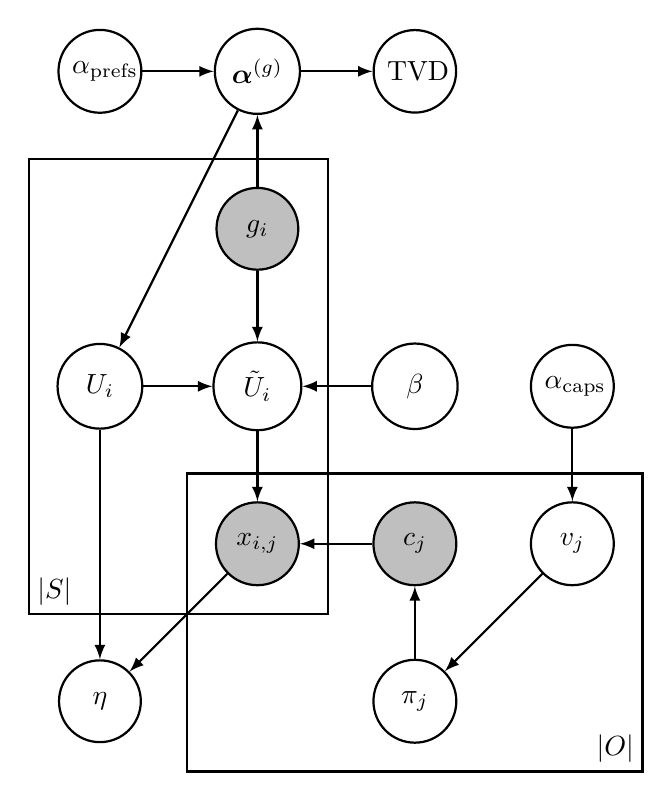
\begin{tikzpicture}
    [
      observed/.style={circle, thick, draw, text width=2em, thick, align=center,fill=gray!50},
      unobserved/.style={circle, thick, draw, text width=2em, align=center},
      arr/.style={->, draw, thick}
    ]
    \node (eta) [unobserved] at (0,0) {$\eta$};
    \node (pi-j) [unobserved] at (4,0) {$\pi_j$};
    \node (x-ij) [observed] at (2,2) {$x_{i,j}$};
    \node (c-j) [observed] at (4,2) {$c_j$};
    \node (v-j) [unobserved] at (6,2) {$v_j$};
    \node (alpha-caps) [unobserved] at (6,4) {$\alpha_{\text{caps}}$}; 
    \node (u-tilde) [unobserved] at (2,4) {$\tilde{U}_i$};
    \node (u-i) [unobserved] at (0,4) {$U_i$};
    \node (beta) [unobserved] at (4,4) {$\beta$};
    \node (g-i) [observed] at (2,6) {$g_i$};
    \node (alpha-prefs) [unobserved] at (0,8) {$\alpha_{\text{prefs}}$};
    \node (alpha) [unobserved] at (2,8) {$\boldsymbol{\alpha}^{(g)}$};
    \node (TVD) [unobserved] at (4,8) {TVD};
    \draw [arr] (alpha-prefs) -- (alpha);
    \draw [arr] (alpha) -- (TVD);
    \draw [arr] (g-i) -- (alpha);
    \draw [arr] (g-i) -- (u-tilde);
    \draw [arr] (u-i) -- (u-tilde);
    \draw [arr] (beta) -- (u-tilde);
    \draw [arr] (alpha) -- (u-i);
    
    \draw [arr] (u-tilde) -- (x-ij);
    \draw [arr] (x-ij) -- (eta);
    \draw [arr] (u-i) -- (eta);
    \draw [arr] (c-j) -- (x-ij);

    \draw [arr] (alpha-caps) -- (v-j);
    \draw [arr] (v-j) -- (pi-j);
    \draw [arr] (pi-j) -- (c-j);

    \node [draw,fit=(g-i) (u-i) (x-ij), inner sep=10pt, thick] (plate-S) {};
    \node [above right] at (plate-S.south west) {$|S|$};
    \node [draw,fit=(x-ij) (v-j) (pi-j), inner sep=10pt, thick] (plate-O) {};
    \node [above left] at (plate-O.south east) {$|O|$};
  \end{tikzpicture}
  %\includegraphics[width=0.9\linewidth]{plate_diagram.pdf}
\caption{Plate diagram of the data generation and matching process. Gender assignments \( g_i \) are sampled from a balanced uniform distribution. For each gender, gender-specific preference priors \( \alpha^{(g)} \) are sampled from a Gamma distribution with parameter \( \alpha_\mathrm{prefs} \), and preferences \( U_i \) are drawn from the corresponding Dirichlet prior. A gender bias \( \beta \) is applied to the preferences of male individuals to favor males over females, resulting in biased preferences \( \tilde{U}_i \). The matching \( x_{ij} \) is determined by solving an ILP that maximizes \( \tilde{U}_i \) under capacity constraints \( c_j \), generated via stick-breaking with \( \alpha_\mathrm{caps} \), \( v_j \), and \( \pi_j \). The optimality \( \eta \) is evaluated using the unbiased preferences \( U_i \). Observable variables are indicated by shaded nodes. Plates represent the number of individuals \( |S| \) and positions \( |O| \).}
\label{fig:plate_diagram}
\end{figure}

\section{Evaluation}

We evaluated the impact of gender bias and quota mechanisms on matching efficiency by systematically combining different levels of discrimination, modeled by a bias adjustment parameter \( \beta \), and quota policies enforcing a female percentage \(q\). Fixed quotas were defined such that \( q \geq T \), where \( T \) could represent predefined thresholds, such as \( T = 20\%\), \( T = 30\%\), or for gender parity, \( T = 50\%\), requiring an exact 50-50 balance between genders. Quotas were implemented as additional linear constraints in the ILP. 

To overcome the limitations of fixed quota thresholds for different gender preferences measured by TVD, we propose and evaluate a new preference-based quota mechanism. This approach aims to better align with average gender-specific preferences while maintaining equitable representation.

To derive the preference-based quota, we consider the scenario where the true and unbiased preferences \( U \) are unknown. Instead, individuals are asked to vote for their single highest preference among the positions. These votes are aggregated separately for females and males to approximate the expectation values of their respective preference priors, \( \mathbb{E}[\textrm{Dirichlet}(\alpha^{(g)})] \) for \( g \in \{f, m\} \). Specifically, the aggregated votes provide empirical estimates of the preference weights for each position, which are then normalized to define the expected preference distribution for each gender:
\[
\hat{\alpha}^{(g)}_j = \frac{\text{Votes for position } o_j \text{ from gender } g}{\text{Total votes from gender } g}.
\]

From these estimated preference distributions, we define the preference-based threshold vector \( \mathbf{T}^{(g)} \) for gender \( g \) and position \( o_j \) as:
\[
T_j^{(g)} = \frac{\hat{\alpha}^{(g)}_j}{\hat{\alpha}^{(f)}_j + \hat{\alpha}^{(m)}_j}.
\]

This mechanism effectively mitigates bias and promotes efficiency by reflecting the actual interests of the groups.

To account for preference divergence, we tracked TVD between gender-specific preferences. This allowed us to analyze the influence of preference divergence on outcomes, particularly when combining fixed and preference-based quota mechanisms.

For our simulation experiments, we performed 100 test runs each with \( \alpha_\text{prefs} = 1 \) and \( \alpha_\text{caps} = 5 \) for 5 positions with a total capacity \( C \) of 100. In each run, a dataset with 250 individuals was generated, including two gender priors with corresponding TVD and individual preferences. For the given number of positions and total capacity, position capacities were generated using the specified parameters. The matching \( \mu \) was then determined for various biases and quotas, which was used to calculate the total and gender-specific efficiencies using the base case of \( \beta = 0 \) and \( q \geq 0\% \) for \(\eta^{\star}\). 

\begin{figure}[ht]
  \centering
  \includegraphics[width=1.0\linewidth]{violin_plot.pdf}
\caption{Violin plots illustrating the total efficiency distribution with bias \( \beta = 0.3 \). The distributions are shown for both high and low TVD scenarios, capturing density and variation within each quota category.}
  \label{fig:violin_plot}
\end{figure}

\section{Results}

Our results highlight the interplay of bias, quotas, TVD, and efficiency in matching scenarios.
In Figure~\ref{fig:violin_plot}, violin plots show efficiency distributions across quota levels for a bias \( \beta = 0.3 \) and scenarios of high and low TVD. For low TVD \( \leq 0.2 \), higher quotas, i.e. \( q\geq 40\%\), compensate the bias quite well and our proposed preference-based quotas achieve comparable efficiency. However, for high TVD~\( \geq 0.8 \), preference-based quotas outperform fixed thresholds by dynamically adapting to preference distributions, resulting in better alignment with group-specific interests and higher overall efficiency. In contrast, strict fixed quotas (e.g., \( q = 50\% \)) significantly reduce efficiency under high TVD due to rigid allocation constraints.

Figure~\ref{fig:scatter_plot} illustrates scatter plots with robust regression lines for varying quota levels and a gender bias \( \beta = 0.2 \). The plots show how TVD, which represents the similarity of preferences, affects efficiency. Without quotas (\( q \geq 0\% \)), higher TVD increases fairness and total efficiency, as a greater divergence between group preferences reduces competition for the same positions and allows for more efficient allocations. Fixed quotas (e.g., \( q \geq 20\%, q \geq 40\% \)) mitigate disparities but do not fully align with group-specific preferences. Although \( q = 50\% \) ensures balanced group outcomes, it can lead to reduced total efficiency under high TVD due to overly rigid constraints. In contrast, our proposed preference-based quotas perform consistently well, dynamically aligning matchings with group preferences, and achieving superior outcomes in fairness and total efficiency.

These findings highlight the advantages of integrating preference-based quotas into matching frameworks, especially under challenging scenarios of biased preferences and high divergence between groups.

\begin{figure}[ht]
  \centering
  \includegraphics[width=1.0\linewidth]{scatter_plot.pdf}
\caption{Scatter plots of efficiency against TVD for bias \( \beta = 0.2 \) and varying quota levels. The plots differentiate total efficiency, male efficiency, and female efficiency, with robust Theil-Sen regression lines included to illustrate trends across quota thresholds.}
  \label{fig:scatter_plot}
\end{figure}

\section{Conclusion}
We present a mathematical framework with a generative process that enables the analysis of gender bias and quotas in many-to-one matching problems through a simulation-based approach. By introducing a bias term and measuring preference divergence via TVD, we quantified how different quota rules mitigate or exacerbate group disparities. Our results show that moderate quotas can improve both fairness and total efficiency when group preferences are similar, whereas strict quotas compromise total efficiency in the face of high divergence. Our novel approach of using votes to derive preference-based quotas achieves the best results and behaves almost independently of the TVD. Future extensions could incorporate more nuanced dimensions of gender and dynamic settings in which individuals adjust their preferences over time.


\bibliographystyle{flairs}
\bibliography{refs}

\end{document}

\cite{lin_why_2017} 
\bigskip
\bibliographystyle{flairs}
\bibliography{refs}
\end{document}